\chapter{El campo electromagnético}

\section{El oscilador armónico}
Comencemos repasando los operadores de creación y destrucción del
oscilador armónico. Tenemos un hamiltoniano
\begin{equation}
  \Ham = \frac{P^2}{2m} + \frac{1}{2}k X^2
\end{equation}
con $\omega = \sqrt{k/m}$. Los autovalores del hamiltoniano son
$E_n=(n+\oh)\hbar\omega$, con $n\in \mathbb{Z}^+$. A los autoestados
(polinomios de Hermite) los denotaremos $\phi_n(x)\coloneqq \ket{n}$.

Definimos los operadores adimensionales
\begin{align}
  \hat{X} &= \sqrt{\frac{m\omega}{\hbar}} X \\
  \hat{P} &= \sqrt{\frac{1}{m\hbar\omega}} P 
\end{align}
con conmutador\footnote{Recordar que $[X,P]=i \hbar$}
$[\hat{X},\hat{P}]=i$. Definimos los \emph{operadores de escalera} $a$ y
$a^\dagger$:
\begin{equation}
  \begin{matrix}
    a = \frac{1}{\sqrt{2}}(\hat{X}+i\hat{P}) \\
    a^\dagger = \frac{1}{\sqrt{2}}(\hat{X}-i\hat{P}) \\
  \end{matrix} \ \leftrightarrow \
  \begin{matrix}
    \hat{X} = \frac{1}{\sqrt{2}}(a^\dagger+a) \\
    \hat{P} = \frac{1}{\sqrt{2}}(a^\dagger-a) \\
  \end{matrix} 
  \label{eq:adef}
\end{equation}
Hay que notar que $a,a^\dagger$ no son hermíticos y por lo tanto no
son observables; no son medibles en un laboratorio. Su conmutador
es $[a,a^\dagger]=1$. Decir que $[a,a^\dagger]=1$ es completamente equivalente a
decir $[\hat{X},\hat{P}]=i$, lo que se suele expresar de manera
formal como un teorema.

\begin{thm}
Dados dos operadores en un espacio de Hilbert tales que su conmutador
es $i$, al definir dos operadores $a$ y $a^\dagger$ como en las
expresiones de la ecuación \eqref{eq:adef} se garantiza que $[a,a^\dagger]$=1.

De forma recíproca, si dados dos operadores $a$ y $a^\dagger$ se
verifica que su conmutador es $[a,a^\dagger] =1$ se tiene que los
operadores $\hat{X}$ y $\hat{P}$ definidos como en \eqref{eq:adef}
cumplirán $[\hat{X},\hat{P}]=i$.
\end{thm}

Reescribamos el hamiltoniano en función de los nuevos operadores
adimensionales:
\begin{equation}
  \begin{split}
    \Ham &= \frac{P^2}{2m} + \frac{1}{2} k X^2 = \frac{1}{2m} m
    \hbar\omega \hat{P}^2 + \frac{1}{2} k \frac{\hbar}{m\omega}
    \hat{X}^2 = \\
    &= \frac{1}{2} \hbar \omega \left( \hat{X}^2 + \hat{P}^2 \right)
  \end{split}
\end{equation}
Notar como ambos operadores son completamente simétricos e
indistinguibles. Desarrollando sus definiciones en términos de $a$ y
$a^\dagger$ se obtiene:
\begin{equation}
\hat{X}^2 + \hat{P}^2 = a^\dagger a + a a^\dagger
\end{equation}
Notar que no se han sumado ambos términos en $2a\cdot a^\dagger$
porque no conmutan. Obtenemos un hamiltoniano
\begin{equation}
  \Ham = \frac{1}{2} \hbar\omega(a^\dagger a + a a^\dagger) = \hbar
  \omega \left( N + \frac{1}{2} \right)
\end{equation}
donde hemos definido el \emph{operador número} $N=a^\dagger a$ y
utilizado las relaciones de conmutación de $a$ y $a^\dagger$. El
operador número actúa sobre un $\ket{n}$ como
$N\ket{n}=n\ket{n}$.\footnote{Ya que
\begin{equation*}
  \begin{split}
    N\ket{n} &= \left( \frac{1}{\hbar \omega}\Ham - \frac{1}{2} \right)\ket{n} = \\
    &= (n+\oh)\ket{n} - \oh\ket{n} = \\
    &= n \ket{n}
  \end{split}
\end{equation*}}

Posee como relaciones de conmutación con los operadores escalera
$[N,a]=-a$ y $[N,a^\dagger]=a^\dagger$, como puede comprobarse fácilmente.

El operador $a^\dagger$ nos permite hallar autoestados superiores del
oscilador armónico a partir del fundamental\footnote{Es una forma compacta de
expresar las relaciones de recurrencia de los polinomios de Hermite}:
\begin{equation}
  N a^\dagger\ket{n} = \cdots = (n+1) a^\dagger \ket{n}
\end{equation}
En una dimensión, y {\bfseries sólo en una dimensión}, se tiene que
$a^\dagger\ket{n}\propto \ket{n+1}, \ \forall n$:
\begin{equation}
  a^\dagger\ket{n} = \sqrt{n+1} \ket{n+1}
\end{equation}
donde se ha elegido por convenio un factor de fase
nulo\jokenote{Cualquier cosa que no sea nula es síntoma de gilipollez.}. Para $a$
obtenemos un resultado similar:
\begin{equation}
  a\ket{n} = \sqrt{n}\ket{n-1}
\end{equation}
En particular, $a\ket{n}=0$.

En la base de los $\{\ket{n}\}$ obtenemos una representación matricial\jokenote{Después de sacar conejos, palomas y cartas de la manga tenemos esto.}
simple para $N,a$ y $a^\dagger$:
\begin{align}
  N &= 
  \begin{pmatrix}
    0& & & & \\
     &1& & & \\
     & &2& & \\
     & & &3& \\
     & & & &\ddots\\
  \end{pmatrix} \tag{Operador número}\\
  a &= 
  \begin{pmatrix}
    0& & & & \\
     \sqrt{1}&0& & & \\
     & \sqrt{2}&0& & \\
     & & \sqrt{3}&0& \\
     & & & \ddots&\ddots\\
  \end{pmatrix} \tag{Operador aniquilación}\\
  a^\dagger &= 
  \begin{pmatrix}
    0&\sqrt{1}& & & \\
     &1&\sqrt{2}& & \\
     & &2&\sqrt{3}& \\
     & & &3&\ddots\\
     & & & & \ddots\\
  \end{pmatrix} \tag{Operador creación}
\end{align}

A los operadores $a,a^\dagger$ se les llama de \emph{creación} y
\emph{destrucción} porque crean o destruyen un cuanto de energía
$\hbar\omega$ (figura \ref{fig:operatora}). En particular, llamamos a
estos cuantos de energía \emph{fonones}, que en el caso del oscilador
armónico tienen todos frecuencia $\omega=\sqrt{k/m}$.
\begin{marginfigure}
  \centering
  \vspace{2cm}
  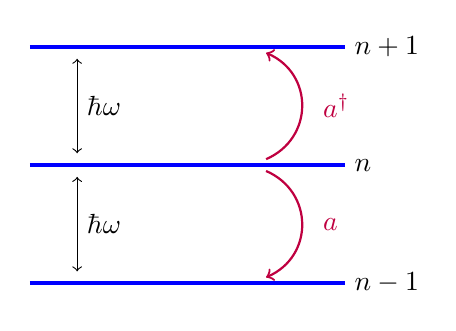
\begin{tikzpicture}[xscale=2,yscale=1.5]
    \draw [ultra thick,blue] (0,0) -- (2,0);
    \draw [ultra thick,blue] (0,1) -- (2,1);
    \draw [ultra thick,blue] (0,2) -- (2,2);
    \draw [<->] (0.3,0.1) -- (0.3,0.9);
    \draw [<->] (0.3,1.1) -- (0.3,1.9);
    \draw [purple, thick, <-] (1.5,0.05) to [out=30,in=-30] (1.5,0.95);
    \draw [purple, thick, ->] (1.5,1.05) to [out=30,in=-30] (1.5,1.95);
    \draw node [right] at (2,0) {$\ket{n-1}$};
    \draw node [right] at (2,1) {$\ket{n}$};
    \draw node [right] at (2,2) {$\ket{n+1}$};
    \draw node [right, purple] at (1.8,0.5) {$a$};
    \draw node [right, purple] at (1.8,1.5) {$a^\dagger$};
    \draw node [right] at (0.3,0.5) {$\hbar\omega$};
    \draw node [right] at (0.3,1.5) {$\hbar\omega$};
  \end{tikzpicture}
  \caption{Efecto de los operadores creación y destrucción}
  \label{fig:operatora}
\end{marginfigure}

Más adelante veremos como el campo electromagnético es similar pero
con fonones en lugar de fotones. El autoestado $\ket{0}$ representa el
vacío (ausencia de fotones), con energía no nula al igual que el
oscilador armónico. El autoestado $\ket{n}$ representa un estado con
$n$ fotones, y una energía $n \hbar\omega$ sobre la energía del vacío.

\section{Campo electromagnético clásico}
Partimos de las ecuaciones de Maxwell\jokenote{El electromagnetismo se caracteriza por tener ecuaciones feas, feas, feas, feas, feas.}:
\begin{center}
  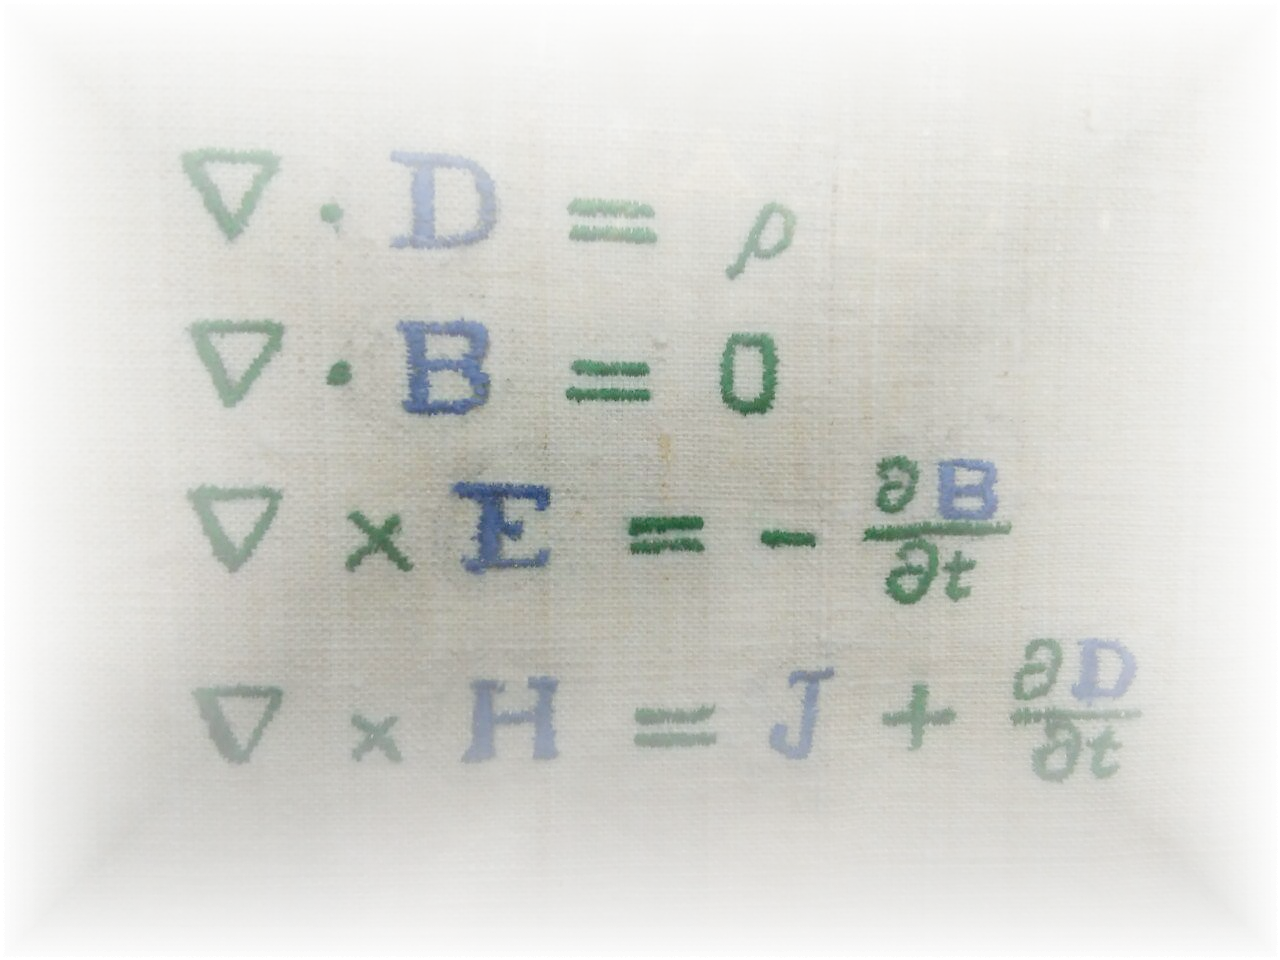
\includegraphics[width=0.6\textwidth]{figures/maxwell.png}
\end{center}

Las ecuaciones homogéneas\footnote{$\nabla \boldrm{D}=0$ y
  $\nabla\times \boldrm{E} + \pdv{\boldrm{B}}{t} = 0$} son fácilmente interpretables como que
$\boldrm{B}$ es el rotacional de un \emph{potencial vector} y
$\boldrm{E}$ un gradiente:
\begin{align}
    \boldrm{B} &= \nabla \times \boldrm{A} \\
  \boldrm{E} &= -\nabla \boldrm{\phi} - \pdv{\boldrm{A}}{t}
\end{align}
Con estas sustituciones podemos reducir las ecuaciones de Maxwell; en el vacío tenemos
\begin{equation}
    \nabla^2 \boldrm{\phi} + \pdv{t} (\nabla \boldrm{A}) =
    \frac{-\rho}{\epsilon_0} 
\end{equation}
y por otra parte\jokenote{Es un ladrillo, naturalmente, como todas las ecuaciones. Pero hay ladrillos bien puestos, veáse la fachada de La Seo.}
\begin{equation}
  \begin{split}
    \nabla^2 \boldrm{A} &= \frac{1}{c^2} \pdv[2]{\boldrm{A}}{t} -
    \nabla \left( \nabla \boldrm{A} + \frac{1}{c^2}
      \pdv{\boldrm{\phi}}{t} \right) = \\
    &= -\mu_0 \boldrm{J}
  \end{split}
  \label{eq:batman}
\end{equation}
Notar que $\nabla^2 \boldrm{A}$ indica tres ecuaciones escalares, no
una. La ventaja de este cambio es que ahora están desacopladas.

Podemos sustituir
\begin{equation}
  \begin{split}
    &\boldrm{A} \ \rightarrow \ \boldrm{A} + \nabla
    \boldrm{\Lambda} \\
    &\boldrm{\phi} \ \rightarrow \ \boldrm{\phi} - \pdv{\boldrm{\Lambda}}{t}
  \end{split}
\end{equation}
y obtenemos los mismos resultados independientemente de la
$\boldrm{\Lambda}(\boldrm{r},t)$\jokenote{Infinitas funciones de este estilo, salvo la función de Diriclhet o alguna parida así.}, a este tipo de transformaciones
se les denomina \emph{transformaciones de gauge}. En particular, para
simplificar la ecuación \eqref{eq:batman}, es interesante escoger el
denominado \emph{gauge de Lorentz}:
\begin{equation}
  - \left( \nabla \boldrm{A} + \frac{1}{c^2}
    \pdv{\boldrm{\phi}}{t} \right) = \nabla^2 \boldrm{\Lambda}
  - \frac{1}{c^2} \pdv[2]{\boldrm{\Lambda}}{t}
\end{equation}
con el que las ecuaciones de Maxwell resultan\footnote{Básicamente,
  con esta elección hacemos que el término $\left( \nabla \boldrm{A} + \frac{1}{c^2}
      \pdv{\boldrm{\phi}}{t} \right)$ de \eqref{eq:batman} sea nulo. }
\begin{equation}
  \begin{split}
    \nabla^2\boldrm{\phi} - \frac{1}{c^2} \pdv[2]{t}
    \boldrm{\phi} &= \frac{-\rho}{\epsilon_0} \\
    \nabla^2 \boldrm{A} - \frac{1}{c^2} \pdv[2]{\boldrm{A}}{t} &=
    -\mu_0 \boldrm{J}
  \end{split}
\end{equation}
de forma que $\boldrm{A}$ se desacopla. La principal ventaja es que es
el mismo para todos los sistemas de referencia. Las fuerzas no cambian
bajo estas transformaciones, ya que dependen de $\boldrm{B}$ y
$\boldrm{E}$, que son invariantes ante estos cambios.
Otra elección es el
\emph{gauge de Coulomb}\jokenote{Habéis estado usando el gauge de
  Coulomb toda la vida. Os hemos estado engañando, pero pasa como con
  los Reyes Magos; mientras dura el engaño se lo pasan muy bien el que engaña y el engañado.}, en que el potencial se propaga de forma
instantánea; si $\boldrm{\phi}=\boldrm{\phi}(t)$ se tiene que
$V\neq V(t)$. Notar que $\boldrm{B},\boldrm{E}$ siguen siendo
  funciones dependientes del tiempo.
Viene de imponer $\nabla \boldrm{A}=0$,
con lo que las ecuaciones quedan
\begin{equation}
  \begin{split}
    \nabla^2 \boldrm{\phi} &= \frac{-\rho}{\epsilon_0} \\
    \nabla^2 \boldrm{A} - \frac{1}{c^2} \pdv[2]{\boldrm{A}}{t} &=
    -\mu_0 \boldrm{J} + \frac{1}{c^2} \nabla \pdv{\boldrm{\phi}}{t}
  \end{split}
  \label{eq:robin}
\end{equation}
El teorema de Helmholtz\footnote{
Wikipedia dixit:
\emph{
Helmholtz's theorem $[\cdots]$ states that any sufficiently smooth, rapidly decaying vector
field in three dimensions can be resolved into the sum of an
irrotational (curl-free) vector field and a solenoidal
(divergence-free) vector field.
}
}\jokenote{Este teorema se llama de nosequién y dice esto} establece en una de sus formas que $\boldrm{J}$ se puede descomponer
en una componente transversal $\boldrm{J}_\perp$ y otra longitudinal
$\boldrm{J}_\parallel$, que verifican $\forall \boldrm{J}$ que  $\nabla
\times \boldrm{J}_\parallel = \boldrm{0}$ y $\nabla \cdot \boldrm{J}=0$.

Con ello y la ecuación de continuidad $\nabla \boldrm{J}+
    \pdv{t}\rho=0$ podemos reescribir las ecuaciones \eqref{eq:robin}
  como\footnote{Utilizamos $\frac{1}{c^2} \nabla
    \pdv{\boldrm{\phi}}{t}=\mu_0 \boldrm{J}_\parallel$, obtenido de
    la ecuacíon de continuidad y de $\nabla^2 \boldrm{\phi} =
    \frac{-\rho}{\epsilon_0}$.} :
  
\begin{equation}
  \begin{split}
    \nabla^2 \boldrm{\phi} &= \frac{-\rho}{\epsilon_0} \\
    \nabla^2 \boldrm{A} - \frac{1}{c^2} \pdv[2]{\boldrm{A}}{t} &=
    -\mu_0 \boldrm{J}_\perp
  \end{split}
  \end{equation}
Vemos que sólo nos importa la componente $\boldrm{J}_\perp$, por ello
al gauge de Coulomb a veces se le denota el \emph{gauge transversal}.
Si $\rho=\abs{\boldrm{J}}=0$ (caso libre) nos queda
  \begin{equation}
  \begin{split}
    \nabla^2 \boldrm{\phi} &= 0\\
    \nabla^2 \boldrm{A} &= \frac{1}{c^2} \pdv[2]{\boldrm{A}}{t} 
  \end{split}
  \end{equation}

\section{Campo electromagnético en el vacío}
Describamos el campo electromagnético de una región del vacío, donde
$\rho=0$ y $\boldrm{J}=0$.\footnote{Evidentemente, fuera de esta
  región de frontera $\rho$ o $\abs{\boldrm{J}}$ no son nulas, ya que
  sino no habría campo alguno.} Utilizaremos el gauge de Coulomb para ello.

Consideremos un campo tal que $\boldrm{\phi}=0$ y $\nabla^2 \boldrm{A}
= \frac{1}{c^2} \pdv[2]{t} \boldrm{A}$. La solución es una
superposición de ondas planas, expresables como
\begin{equation}
  \boldrm{A}_\lambda e^{-i\omega_\lambda t} = L^{-\nicefrac{3}{2}}
  \boldrm{\Pi}_\lambda e^{i \boldrm{k}_\lambda \boldrm{r}} e^{-i
    \omega_\lambda t} 
\end{equation}
donde $\boldrm{\Pi}$ es el vector de polarización y $\omega_\lambda =
\abs{\boldrm{k}_\lambda}c$, con condiciones de normalizacion $\iiint \dd{V}
\abs{\boldrm{A}_\lambda}^2 =1$.

Utilizando que en el gauge de Coulomb $\nabla \boldrm{A} = 0$ y
omitiendo por simplicidad los subíndices $\lambda$, se tiene para
$\hat{x}$
\begin{equation}
  \pdv{A_x}{x} = \pdv{x} \left( \Pi_x e^{i \boldrm{k}
      \boldrm{r}} \right) = \Pi_x (ik_x) e^{i \boldrm{k}\boldrm{r}}
\end{equation}
El cálculo para $\hat{y}, \hat{z}$ es análogo; sumando las tres
derivadas parciales (operador divergecia) se tiene
\begin{equation}
  \nabla \boldrm{A} = i (\Pi_x k_x + \Pi_y k_y + \Pi_z k_z) e^{i \boldrm{k}\boldrm{r}} = 0
  \ \rightarrow \ \boldrm{\Pi} \perp \boldrm{k}
\end{equation}
La solución general para $\boldrm{A}$ es
\begin{equation}
  \boldrm{A}(\boldrm{r},t) = \sum_{\lambda} \left( q_\lambda
    \boldrm{A}_\lambda e^{-i\omega_\lambda t} + q_\lambda^*
    \boldrm{A}_\lambda^* e^{i \omega_\lambda t} \right) \in \mathbb{R}
  \label{eq:aform}
\end{equation}
Es un número real, por lo que $\boldrm{E}$ y $\boldrm{B}$ también lo
son. En particular, para $\boldrm{E}$ se tiene
\begin{equation}
  \boldrm{E} = \frac{1}{c} \pdv{\boldrm{A}}{t} =
 \frac{-i}{c}\sum_{\lambda}  \omega_\lambda\left( q_\lambda
    \boldrm{A}_\lambda e^{-i\omega_\lambda t} - q_\lambda^*
    \boldrm{A}_\lambda^* e^{i \omega_\lambda t} \right) \in \mathbb{R}
\end{equation}
$\boldrm{B}$ se obtiene fácilmente como $\nabla\times \boldrm{A}$.

\subsection{Energía}

La energía del sistema es (en CGS):
\begin{equation}
  E = \frac{1}{8\pi} \iiint_{L^3} \dd{V} \left( \boldrm{E}^2 + \boldrm{B}^2 \right)
\end{equation}

Calculemos los términos. Podemos expresar $\boldrm{E}^2$ como
\begin{equation}
  \boldrm{E}^2 =  \frac{1}{c^2} \left( \sum_{\lambda} \cdots \right) \left( \sum_{\lambda'} \cdots \right)
\end{equation}

Comenzamos por los términos directos, en los que $\lambda=\lambda'$.

\begin{equation}
  \frac{-\omega}{c^2} \left( q^2 \boldrm{A} \boldrm{A}
    e^{-2i\omega t} + q^{*2} \boldrm{A}^*  \boldrm{A}^*
    e^{2i\omega t} - qq^* \boldrm{A}\boldrm{A}^* - q^*q \boldrm{A}^* \boldrm{A} \right)
\end{equation}
Recordando que $\boldrm{A}=L^{-\nicefrac{3}{2}} \boldrm{\Pi} e^{i
  \boldrm{k}\boldrm{r}}$ vemos que $\boldrm{A}\boldrm{A}^* = L^{-3}
\underbrace{\abs{\Pi}^2}_{=1} = \boldrm{A}^* \boldrm{A}$, y que
$\boldrm{A}\boldrm{A} = L^{-3} \abs{\boldrm{P}}^2 e^{2 i
  \boldrm{k}\boldrm{r}}$. La integral de $\boldrm{A}\boldrm{A}$
quedará como
\begin{equation}
  \iiint_{L^3} \dd{V} \boldrm{A} \boldrm{A} = \int_0^L \dd{x} e^{2i
    k_x x} \int_0^L \dd{y} e^{2i
    k_x y}  \int_0^L \dd{z} e^{2i
    k_x z}
\end{equation}
donde los términos son nulos por las condiciones de
contorno\footnote{En cada integral se obtiene $\eval{\frac{1}{2ik_x}
    \exp(i2k_xx)}_0^L$, pero las condiciones de contorno periódicas
  anulan estos términos (valen lo mismo en $0$ y en $L$).}.

Para los términos cruzados $\lambda\neq\lambda'$ se obtiene
\begin{equation}
  \begin{split}
    \frac{-\omega\omega'}{c} \Big[& qq' \boldrm{A}\boldrm{A}'
    e^{-i(\omega+\omega')t} + q^* q'^{*} \boldrm{A}^*
    \boldrm{A}'^{*} e^{i(\omega+\omega')t} -\\
    &- q q'^* \boldrm{A} \boldrm{A}^{*} e^{-i(\omega-\omega')t} - q^*
    q' \boldrm{A}^* \boldrm{A}' e^{i(\omega-\omega')t} \Big]
  \end{split}
\end{equation}

Por las mismas razones que antes, las integrales $\iiint
\boldrm{A}\boldrm{A}$ se cancelan.

Las integrales finales quedan
\begin{equation}
  \iiint_{L^3} \frac{1}{8\pi} \boldrm{E}^2 \dd{V} = \iiint_{L^3}
  \frac{1}{8\pi}\boldrm{B}^2 \dd{V} = \frac{\omega^2}{c^2} (q^* q + q ^*)
\end{equation}
y obtenemos que la energía es
\begin{equation}
  E = \frac{1}{4\pi c^2} \sum_{\lambda} \omega_\lambda^2 q_\lambda^* q_\lambda
\end{equation}
Definimos las nuevas variables ``posición'' y ``momento'', por
analogía\footnote{Se omite la demostración}:
\begin{align}
 Q_\lambda &= \frac{1}{\sqrt{4\pi c^2}}
(q^*_\lambda + q_\lambda) \\
P_\lambda &= \frac{i\omega_\lambda}{\sqrt{4\pi c^2}}
(q^*_\lambda - q_\lambda)
\end{align}
Obtenemos un hamiltoniano similar al de un
oscilador armónico:
\begin{equation}
  \Ham = \sum_{ \lambda} \frac{1}{2} \left( P_\lambda^2 +
    \omega_\lambda^2 Q_\lambda^2  \right)
  \label{eq:oscilatorem}
\end{equation}
\subsection{Cuantificación}
Vemos en \eqref{eq:oscilatorem} que el campo electromagnético se puede modelar como un conjunto
de osciladores armónicos independientes. La energía es simplemente la
suma de las energías de cada ``oscilador'' (figura \ref{fig:muellefotonico}):
\begin{equation}
  E = \sum_{ \lambda} \left( n_\lambda + \frac{1}{2} \right) \hbar\omega_\lambda
\end{equation}
\begin{marginfigure}
  \begin{tikzpicture}
    \tikzstyle{boing}=[snake=coil, line after snake=0.1cm
    , line before snake = 0.1cm
    , segment amplitude = 0.15cm]
    % Draw the balls
    \node[circle,fill=blue,inner sep=2.5mm] (a) at (1.5,4) {};
    \node[circle,fill=blue,inner sep=2.5mm] (b) at (3,3) {};
    \node[circle,fill=blue,inner sep=2.5mm] (c) at (2,2) {};
    % Draw the springs
    \draw[boing, segment length = 0.5mm] (0.5,4) to (a);
    \draw[boing, segment length = 2mm] (0.5,3) to (b);
    \draw[boing, segment length = 1mm] (0.5,2) to (c);
    % Labels
    \node[right] (a) at (3.5,3) {$x_2,m_2,k_2$};
    \node[right] (a) at (2,4) {$x_1,m_1,k_1$};
    \node[right] (a) at (2.5,2) {$x_3,m_3,k_3$};
    % Wall
    \fill [color=black!20] (0.2,1) rectangle (0.5,5);
    \draw[ultra thick] (0.5,1) -- (0.5,5);
  \end{tikzpicture}
  \caption{Modelizado del campo EM como un conjunto de osciladores}
  \label{fig:muellefotonico}
\end{marginfigure}
con autoestados $\ket{n_{\lambda1}} \otimes \ket{n_{\lambda2}} \otimes
\cdots$ que dan cuenta de los \emph{números de ocupación} o número de
fotones de cada $\lambda_i$.\footnote{Se suelen escribir como 
  \begin{equation*}
    \ket{n_{\lambda1},n_{\lambda2},n_{\lambda3},\cdots}
  \end{equation*}
}

Definimos los operadores de creación y destrucción:
\begin{align}
  a_\lambda^\dagger &= \frac{1}{\sqrt{2 \hbar\omega_\lambda}}
  (\omega_\lambda Q_\lambda - i P_\lambda) =
                      \sqrt{\frac{\omega_\lambda}{2\pi \hbar c^2}} q_\lambda^*\\
  a_\lambda&= \frac{1}{\sqrt{2 \hbar\omega_\lambda}}
  (\omega_\lambda Q_\lambda + i P_\lambda) =
                      \sqrt{\frac{\omega_\lambda}{2\pi \hbar c^2}} q_\lambda
\end{align}
Es inmediato que $[a^\dagger,a]=1$. Además,
$[a_\lambda,a_{\lambda'}^\dagger]=0$ al actuar en espacios distintos.

El efecto de los operadores de creación y destrucción es
idéntico al
del caso del oscilador armónico:
\begin{align}
  a_\lambda^\dagger \ket{\cdots,n_\lambda,\cdots} &=
                                                    \sqrt{n_\lambda+1}\ket{\cdots,n_\lambda+1,\cdots} \\
  a_\lambda \ket{\cdots,n_\lambda,\cdots} &= \sqrt{n_\lambda}\ket{\cdots,n_\lambda-1,\cdots}
\end{align}
Hay que recordar que hay que extender los operadores con la
  identidad. Por ejemplo,\[a_3 \coloneqq \mathbb{I}\otimes 
    \mathbb{I}\otimes a_3\otimes  \mathbb{I} \otimes \cdots \]

De igual forma, podemos definir el operador número $N$ como $N_\lambda
= a_\lambda^\dagger a_\lambda$, obteniendo
\begin{equation}
  \Ham = \sum_{\lambda} \hbar \omega_\lambda \left( N_\lambda + \frac{1}{2} \right)
\end{equation}
El inconveniente de esta formulación es que la energía del vacío,
$\ev{\Ham}{0}$, es infinita\footnote{Esto es debido a que los kets
  tienen infinitos elementos, y el sumatorio corre sobre infinitos
  términos.}. Resolvemos este problema con la siguiente
renormalización:
\begin{equation}
  \Ham = \sum_{\lambda} \hbar\omega N_\lambda
\end{equation}
de forma que $\ev{\Ham}{0}=0$.

\section{Interacción del campo EM con la materia}
Consideramos el campo EM creado por cargas al moverse, y como influye
en su movimiento; el sistema típico a estudio es el átomo. Utilizamos
como sistema de referencia inercial el núcleo, por su escaso
movimiento, y escribimos el hamiltoniano\footnote{Es un hamiltoniano
  propuesto por Fermi, en sistema CGS y con el gauge de Coulomb. En \emph{Mecanique quantique}, de Claude Cohen-Tannoudji, hay una explicación exhaustiva de la elección.} del sistema:
\begin{equation}
  \Ham = \frac{1}{2m} \left( \boldrm{p}_i - \frac{e_i}{c}
    \boldrm{A}_\perp (\boldrm{r}_i) \right)^2 + \sum_{i<j}
  \frac{e_ie_j}{\abs{\boldrm{r}_i - \boldrm{r}_j}} + \Ham_\text{EM}(\boldrm{A}_\perp)
  \label{eq:hamiltonrules}
\end{equation}
Notar que no es un hamiltoniano de partículas independientes. 

Si consideramos una sola carga y las ecuaciones de Hamilton\footnote{
  \begin{align*}
    \dot{p} &= \pdv{\Ham}{q}\\
    \dot{q} &= \frac{-\partial \Ham}{\partial p}
  \end{align*}
} obtenemos la fuerza de Lorentz. El desarrollo concreto puede
consultarse en \emph{Mecanique quantique}, de Claude Cohen-Tannoudji.

Consideremos un átomo, en el que $e_i=-e$ y $m_i=m$, con la masa del
núcleo aproximable a infinita. El hamiltoniano \eqref{eq:hamiltonrules} queda como
\begin{equation}
  \begin{split}
  \Ham &= 
  \textcolor{red!60!black}{
  \sum_{i=1}^N \frac{p_i^2}{2m} + V 
  }
  + \\
  &+ 
  \textcolor{blue!60!black}{
  \frac{e}{2mc} \sum_{i=1}^N \left[ \boldrm{p}_i
    \boldrm{A}(\boldrm{r}_i,t) + \boldrm{A}(\boldrm{r}_i,t) \boldrm{p}_i \right]+
    \frac{e^2}{2mc^2} \sum_{i=1}^N \boldrm{A}^2(\boldrm{r}_i,t)
    }
  + \\
    &+
    \textcolor{green!60!black}{
 \Ham_\text{EM}
 }
  \end{split}
  \label{eq:aynomames}
\end{equation}
Por lo que tenemos $\Ham = 
 \textcolor{red!60!black}{\Ham_\text{at.}}
+\textcolor{blue!60!black}{\Ham_\text{int}}
+\textcolor{green!60!black}{\Ham_\text{EM}}$. Definimos $\Ham_0 =
\Ham_\text{at.}+\Ham_\text{EM}$, de forma que $\Ham =
\Ham_0+\Ham_\text{int}(t)$. Notar que falta el término de interacción
con el espín\footnote[][-3cm]{Sería un término extra de la
  forma \[\sum_{i}-\boldrm{\mu}_i(\boldrm{\Pi}\times \boldrm{A})\]No
  es necesario incluirlo ya que cortaremos la aproximación en primer
  orden (dipolo eléctrico) y ahí no entra el término de espín.}.

\subsection{Aproximación perturbativa de la emisión espontánea}
La probabilidad de que en el átomo se produzca una emisión espontánea
de un fotón viene dada por
\begin{equation}
  P_{if}(t) = \frac{1}{\hbar^2} \abs{\int_0^t
    \mel{\phi_f}{\Ham_\text{int}(\tau)}{\phi_i} e^{i\omega_{fi}\tau}\dd{\tau} }^2 
  \label{eq:probaif}
\end{equation}
Caracterizamos al estado inicial $\phi_i$ como $\ket{I}$ y al final
$\phi_f$ como $\ket{F}$ para aliviar la notación. En función de sus
valores, tenemos distintos fenómenos físicos:
\marginnote{Para aliviar la notación, se empleará a partir de ahora
  $\ket{\cdots,a,\cdots}\equiv\ket{a}$,
  $\ket{\cdots,a,b,\cdots}\equiv\ket{a,b}$, etc. Se sobreentienden las
componentes no nombradas del autoestado.} 
\begin{itemize}
\item Si $\ket{I}=\ket{1_\lambda}$ y
  $\ket{F}=\ket{0_\lambda}$, se ha absorbido un fotón.
\item Si en cambio $\ket{F}=\ket{1_\lambda}$ y
  $\ket{I}=\ket{0_\lambda}$, estamos ante la emisión
  espontánea de un fotón por el átomo.
\item Para $\ket{I}=\ket{1_\lambda}$, si se tiene
  emisión inducida por el fotón $1_\lambda$ se obtendrá
  $\ket{F}=\ket{2_\lambda}$ (se excita un fotón de
  idéntica longitud de onda) o
  $\ket{F}=\ket{1_\lambda,1_{\lambda'}}$ (el fotón
  excitado es de distinta $\lambda$).
\end{itemize}

Para calcular la integral \eqref{eq:aynomames} necesitamos ver si
$\boldrm{A}$ y $\boldrm{p}$ conmutan:
\begin{equation}
  \begin{split}
    (\boldrm{p}\boldrm{A}) \boldrm{\phi} &= -i \hbar \nabla (\boldrm{A}\boldrm{\phi}) =
    \\
    &= \left( \pdv{x} A_x\boldrm{\phi} +  \pdv{y} A_y\boldrm{\phi}+ \pdv{z} A_z\boldrm{\phi}
    \right) =\\
    &= -i \hbar \left[ (\nabla \boldrm{A})\boldrm{\phi}+ \boldrm{A}\nabla \boldrm{\phi}
    \right] = \\
    &= (\boldrm{A}\boldrm{p})\boldrm{\phi} 
  \end{split}
\end{equation}

De donde de vemos que el término
$\boldrm{p}\boldrm{A}+\boldrm{A}\boldrm{p}$ de \eqref{eq:aynomames} es
simplemente $2 \boldrm{A}\boldrm{p}$. Utilizando la ecuación
\eqref{eq:aform} para $\boldrm{A}$ vemos que el primer sumando de $\Ham_\text{int}$ 
puede escribirse como
\begin{equation}
  \begin{split}
    \frac{e}{2mc} \sum_{i} \left[ \boldrm{p}_i \boldrm{A} +
      \boldrm{A}\boldrm{p} \right] &= 2\cdot\frac{e}{2mc} \sum_{i} \sum_{\lambda} \Big[
    \mel{F}{\boldrm{A}_{\lambda'}\boldrm{p}_i e^{-i\omega'_\lambda
        t}}{I} \mel{n_\lambda = 1}{q_{\lambda'}}{0} +  \\
    &+
\mel{F}{\boldrm{A}_{\lambda'}^*\boldrm{p}_i e^{i\omega'_\lambda
        t}}{I} \mel{n_\lambda = 1}{q_{\lambda'}^\dagger}{0} \Big]= \cdots
  \end{split}
\end{equation}
donde estamos suponiendo situación de emisión espontánea. El término
$\mel{n_\lambda=1}{q_\lambda'}{0}$ se anula, ya que se aplica el
operador destrucción al vacío, $\ket{0}$. El segundo término se puede
reescribir en función del operador creación utilizando que $q_{\lambda'}^\dagger\ket{0} = \left(
  \frac{2\pi \hbar c^2}{\omega_{\lambda'}}
\right)^2\cdot1\ket{n_{\lambda'}=1}$. De esta forma, nos quedan
términos
$\ket{n_\lambda=1}{n_{\lambda'}=1}=\delta_{\lambda,\lambda'}$, que
eliminan todos los $\lambda'$ del sumatorio excepto $\lambda$:

\begin{equation}
  \begin{split}
    \cdots &= \sum_{i} \frac{e}{mc} \sqrt{ \frac{2\pi \hbar
        c^2}{\omega_\lambda} }  
\mel{F}{\boldrm{A}_{\lambda'}^*\boldrm{p}_i }{I} e^{i\omega'_\lambda
        t}
  \end{split}
\end{equation}

Para el otro término de $\Ham_\text{int}$, que depende de
$\boldrm{A}^2$, tenemos un doble sumatorio (uno por cada
$\boldrm{A}$). No obstante, vemos que es nulo al aparecer varios
braket $\braket{I}{F}=\braket{1_\lambda}{0}$:
\begin{itemize}
\item Los elementos $q_{\lambda'}q_{\lambda''}\ket{0}$ son nulos al
  aplicarse el operador destrucción al vacío.
\item Para los términos creación-destrucción se tiene
\begin{equation}
  \mel{1_\lambda}{q_{\lambda'}q^\dagger_{\lambda''}}{0} \sim
  \braket{1_\lambda}{1_{\lambda'}1_{\lambda''}} = 0
\end{equation}
que se anula porque los osciladores son independientes.
\item El término
  $\mel{1_\lambda}{q_{\lambda'}q_{\lambda''}^\dagger}{0} \sim
  \mel{1_{\lambda'}}{q_{\lambda'}}{1_{\lambda''}}$ puede actuar sobre
  una coordenada no vacía ($\braket{1_\lambda}{0}=0$) o sobre una
  coordenada vacía, en cuyo caso resulta nulo al estar aplicándose $q$ a $\ket{0}$.
\end{itemize}

Con todo lo visto, la probabilidad \eqref{eq:probaif} de emisión
espontánea queda
\begin{equation}
  P_{if} = \frac{1}{\hbar^2} \frac{e^2}{m^2c^2} \left( \frac{2\pi
      \hbar c^2}{\omega_\lambda} \right) \abs{\mel{F}{\textstyle \sum \displaystyle
      \boldrm{A}_\lambda^*(\boldrm{r}_i)\boldrm{p}_i}{I}}^2
  \abs{F(\omega_{fi}+\omega_\lambda,t)}^2
  \label{eq:machete}
\end{equation}
donde 
\begin{equation}
F(\omega_{fi}+\omega_\lambda,t) = \int_0^t
e^{i(\omega_{fi}+\omega_\lambda)t'} = \left[ \frac{\sin[(\omega_{fi}+\omega_\lambda)\frac{t}{2}]}{\frac{1}{2}(\omega_{fi}+\omega_\lambda)} \right]^2
\end{equation}
$F$ tiene un límite asintótico en $t\to\infty$ dado por
$\lim_{t\to\infty}\frac{\sin^2\alpha t}{\alpha^2}=\pi t \cdot
\delta(\alpha)$. Sustituyendo este resultado y diviendo entre $t$ la
ecuación \eqref{eq:machete} hallamos la probabilidad de transición por
unidad de tiempo $\Lambda_{fi}$:
\begin{equation}
  \Lambda_{fi} = \frac{2\pi}{\hbar} \abs{H_{fi}}^2 \delta(E_{fi}+E_\lambda)
\end{equation}
con dimensiones de inversa de
tiempo\footnote{$[\delta(E_{fi}+E_\lambda)]=E^{-1}$. Puede verse en
  ejemplos como $\int_{\mathbb{R}}\delta(x)\dd{x}=1$}. Notar que la
delta de Dirac refleja un resultado ya conocido, que la energía del
fotón tiene que coincidir con la $\Delta E$ entre niveles para que se
efectúe una transición.

El fotón tiene un momento $\boldrm{k}_\lambda$ dentro de un continuo;
la probabilidad de encontrar uno con un momento exacto es nula.
Queremos calcular sumas del estilo $\sum_{f}\Lambda_{if}$ para ver la
probabilidad de transición total de un nivel dado, para ello
recurrimos a calcular la \emph{densidad de estados}, transformándose
la suma en una integral.
Se utilizan condiciones de contorno periódicas en
el borde de cada cubo del $k$-espacio ($e^{ik_x0}=e^{ik_xL}=1$), de forma que
\begin{equation}
  k_{x_i} = n_{x_i} \frac{2\pi}{L}; \ \ n_{x_i} \in \{\pm1,\pm2,\cdots\}
\end{equation}
donde $x_i \in \{x,y,z\}$. De esta forma, quedan definidos sucesivos
nodos cúbicos separados $\frac{2\pi}{L}$ en los ejes, correspondiendo
cada nodo a una $\boldrm{k}$ (figura \ref{fig:nodoloco}).


\begin{marginfigure}
  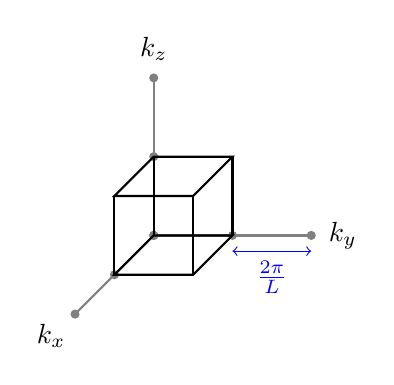
\begin{tikzpicture}[xscale=1,yscale=1]
    % y axis
    \draw [thick,gray] (0,0) -- (2,0);
    \draw [gray,fill] (0,0) circle (0.05);
    \draw [gray,fill] (1,0) circle (0.05);
    \draw [gray,fill] (2,0) circle (0.05);
    \draw node [right] at (2.1,0) {$k_y$};
    % z axis
    \draw [thick,gray] (0,0) -- (0,2);
    \draw [gray,fill] (0,0) circle (0.05);
    \draw [gray,fill] (0,1) circle (0.05);
    \draw [gray,fill] (0,2) circle (0.05);
    \draw node [above] at (0,2.1) {$k_z$};
    % x axis
    \draw [thick,gray] (0,0) -- (-1,-1);
    \draw [gray,fill] (0,0) circle (0.05);
    \draw [gray,fill] (-0.5,-0.5) circle (0.05);
    \draw [gray,fill] (-1,-1) circle (0.05);
    \draw node [below left] at (-1,-1) {$k_x$};
    % cube bottom
    \draw [thick, black]
     (0,0) -- (1,0) -- (0.5,-0.5) -- (-0.5,-0.5) -- (0,0);
    % cube top
    \draw [thick, black]
     (0,1) -- (1,1) -- (0.5,+0.5) -- (-0.5,+0.5) -- (0,1);
    % cube walls
     \draw [thick,black] (0,0) -- (0,1);
     \draw [thick,black] (1,0) -- (1,1);
     \draw [thick,black] (-0.5,-0.5) -- (-0.5,0.5);
     \draw [thick,black] (+0.5,-0.5) -- (+0.5,0.5);
    % some labels
     \draw [thin,blue, <->] (1,-0.2) -- (2,-0.2);
    \draw node [below,blue] at (1.5,-0.2) {$\frac{2\pi}{L}$};
  \end{tikzpicture}
  \caption{$k$-espacio de integración. Se muestra un nodo cúbico
    correspondiente a una $\boldrm{k}$.}
  \label{fig:nodoloco}
\end{marginfigure}

Un diferencial de volumen del $k$-espacio correspondrá a
$\frac{k^2}{(2\pi/L)^3}\dd{k}\dd{\Omega}$ nodos
$\boldrm{k}$\footnote{Se ha efectuado un cambio a coordenadas polares;
$k^2 \dd{k} \dd{\Omega}$ es equivalente al típico $\dd{V}=r^2 \dd{r} \sin{\theta}\dd{\theta}$.};
relacionando $\abs{\boldrm{k}}$ con la energía se tiene
\begin{equation}
  E = \hbar c k = \left( \frac{L}{2\pi} \right)^3 \frac{E^2}{(\hbar
    c)^3} \dd{E} \dd{\Omega}
\end{equation}
Calculamos la densidad de estados como $\rho(E) = E/\dd{E}$:
\begin{equation}
  \rho(E_\lambda) = \left( \frac{L}{2\pi} \right)^3 \frac{E^2}{(\hbar
    c)^3} \dd{\Omega}
\end{equation}

Ahora, ya estamos en condiciones de calcular la suma:
\begin{equation}
  \begin{split}
    \sum_{f} \Lambda_{if} &= \int_\star \dd{E_\lambda}
    \frac{2\pi}{\hbar} \abs{\Ham_{fi}}^2 \delta(E_{fi}+E_\lambda)
    \rho(E_\lambda) =\\
    &= \frac{2\pi}{\hbar}\abs{\Ham_{fi}}^2 \rho(E_\lambda)
  \end{split}
\end{equation}

Donde $\rho(E_\lambda) = \rho(E_{fi})$. La región de integración
abarca el rango de la instrumentación utilizada, por ejemplo de
\SI{300}{\nano\metre} a \SI{600}{\nano\metre} y un ángulo sólido
correspondiente a media esfera. 




\subsection{Aproximación dipolar eléctrica}
\marginnote{Seguimos considerando emisión espontánea}Para poder aplicar esta aproximación se ha de cumplir que
$\lambda=\frac{2\pi}{k_\lambda}$ sea muy inferior al tamaño del átomo,
verificándose en tal caso que en sus vecindades $e^{-i
  \boldrm{k}\boldrm{r}}\simeq 1$.

Veamos el valor de la contribución
$\mel{F;n_\lambda=1}{-\boldrm{\mu}_s (\nabla\times \boldrm{A})}{I}$ del espín al hamiltoniano, antes
despreciado:
\begin{equation}
  \nabla\times \boldrm{A} = i \sum_{\lambda} \boldrm{k}_\lambda\times
  (q_\lambda \boldrm{A}_\lambda e^{-i\omega_\lambda t} +
  q_\lambda^\dagger \boldrm{A}_\lambda^* e^{i\omega_\lambda t})
\end{equation}
El primer término del producto vectorial aplicado en el elemento de
matriz del espín será del estilo $q\ket{I}=q\ket{0}$, siendo por
tanto nulo. El segundo nos dará un braket
$\braket{n_\lambda}{n_{\lambda'}} \sim \delta_{\lambda,\lambda'}$, eliminando todos los términos del
sumatorio salvo uno. Obtenemos:
\begin{equation}
  \mel{F}{-\boldrm{\mu}_s e^{i \boldrm{k}_\lambda \boldrm{r}_i } (i
    \boldrm{k}_\lambda \times \boldrm{\Pi}_\lambda) e^{i
      \omega_\lambda t}}{I}
\end{equation}
Expresando el momento magnético en función del
espín\footnote{$\boldrm{\mu}_s = g_s \mu_{\scriptstyle B}
  \frac{\boldrm{s}}{\hbar}\simeq 2 \mu_{\scriptstyle B}
  \frac{\boldrm{s}}{\hbar} = \frac{e}{mc} \boldrm{s}$} obtenemos
\begin{equation}
  \mel{F}{
    \sum_{i} \boldrm{S}_i (\boldrm{k}_\lambda \times
    \boldrm{\Pi}_\lambda) \underbrace{e^{-i \boldrm{k}_\lambda
        \boldrm{r}_i}}_{\simeq 1}
}{I}
\end{equation}
Se puede comparar con el elemento del dipolo eléctrico y ver que es
claramente inferior:
\begin{equation}
  \frac{\mel{F}{\boldrm{\Pi}_\lambda
      \boldrm{p}_i}{I}}{\mel{F}{\boldrm{s}_i (\boldrm{k}_\lambda
      \times \boldrm{\Pi}_\lambda)}{I}} = \frac{mv
    \frac{R}{R}}{\frac{\hbar}{2} \frac{1}{\lambda}} \sim \frac{\hbar
    \frac{1}{R}}{\hbar \frac{1}{\lambda}} \sim \frac{\lambda}{R} \gg 1
\end{equation}

Por tanto utilizaremos el hamiltoniano
\begin{equation}
  \Ham_{at.} = \sum_{i} \frac{p_i^2}{2m} + \sum_{i} \frac{Ze^2}{r_i} +
  \sum_{i<j} \frac{e^2}{r_{ij}}
\end{equation}
Calculamos el conmutador de $x_i$ con $\Ham_\text{at.}$:
\begin{equation}
  \begin{split}
    [x_i,\Ham_\text{at.}] &= \frac{1}{2m} [x_i,p_i^2] =
    \frac{1}{2m}[x_i,p_{ix}^2] = \\
    &= \frac{1}{2m} ([x_i,p_{ix}]p_{ix}+p_{ix}[x_i,p_ix]) = \frac{2i
      \hbar p_{ix}}{2m}
  \end{split}
\end{equation}
donde se ha utilizado que $[x_i,p_{ix}]=i \hbar$. Obtenemos:
\begin{equation}
  [\boldrm{r}_i,\Ham_\text{at.}] = i \hbar \frac{\boldrm{p}_i}{m}
\end{equation}
y por lo tanto $\boldrm{p}_i =
\frac{im}{\hbar}[\Ham_\text{at.},\boldrm{r}_i]$. Introduciendo esto en
el elemento de matriz, obtenemos la probabilidad de emisión espontánea
de un fotón, que está notablemente simplificada respecto a \eqref{eq:machete}:
\begin{equation}
 \Lambda_{if} = \frac{e^2}{2\pi \hbar}
 \underbrace{\frac{E_\lambda^2}{(\hbar c)^3 }E_\lambda}_{k^3}
 \abs{\mel{F}{\boldrm{\Pi}_\lambda \textstyle \sum_i \displaystyle
     \boldrm{r}_i}{I}}^2 \dd{\Omega}
\end{equation}
Es inmediato ver que $\mel{F}{\boldrm{\Pi}\boldrm{R}}{I} =
\boldrm{\Pi}\mel{F}{\boldrm{R}}{I}$,donde $\boldrm{R}_i =
\sum_{i}\boldrm{r}_i$. Con esto, obtenemos
\begin{equation}
  \Lambda_{if} = \frac{e^2}{2\pi \hbar} k^3
  \abs{\mel{F}{\boldrm{R}}{I}\cdot \boldrm{\Pi}}^2 \dd{\Omega}
\end{equation}
\marginnote[-2cm]{A partir de ahora se omitirán los subíndices $\lambda$,
  sobreentendiéndose.}

Los fotones emitidos tienen una polarización $\boldrm{\Pi}$ en un
diferencial de ángulo sólido $\dd{\Omega}$. Como el elemento de matriz
puede ser complejo, se puede definir como
\begin{equation}
  \mel{F}{\boldrm{R}}{I} = \boldrm{R}' + i \boldrm{R}''
\end{equation}
con $\boldrm{R}',\boldrm{R}''\in \mathbb{R}^3$. Podemos pintar estos dos vectores en un triedro (figura \ref{fig:triedro}).
\begin{marginfigure}
  \centering
  \vspace{2cm}
  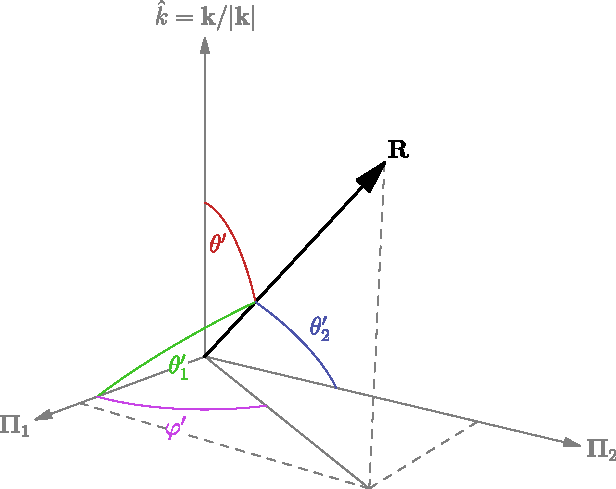
\includegraphics[width=\textwidth]{figures/triedro.pdf}
  \caption{Triedro de la parte real del elemento de matriz del campo
    EM. El elemento imaginario es similar; ponemos
  dos tildes a sus coordenadas para identificarlas en lugar de una sola.}
  \label{fig:triedro}
\end{marginfigure}
El ángulo que forma $\boldrm{R}'$ con una polarización $\boldrm{\Pi}_i$ será del
estilo $\boldrm{R}'\cdot \boldrm{\Pi}_i =
\cos(\theta'_i)|\boldrm{R}'|$, de forma que obtenemos para las dos
polarizaciones ortogonales posibles
\begin{align}
  \cos(\theta'_1) &= \sin(\theta')\cos(\varphi')
  \label{eq:mini1} \\
  \cos(\theta'_2) &= \sin(\theta')\sin(\varphi')
  \label{eq:mini2}
\end{align}
Para $\boldrm{R}''$ obtenemos lo mismo pero con dos tildes \verb~'~ en lugar de una.
Supuesta polarización en $\boldrm{\Pi}_1$,
\begin{equation}
  \Lambda_{if} = \frac{e^2}{2\pi \hbar}k^3 (\abs{\boldrm{R}'}^2
  \cos^2\theta'_1 + \abs{\boldrm{R}''}^2
  \cos^2\theta''_1) \dd{\Omega}
\end{equation}
Suponiendo que no estamos interesados en medir la polarización, sólo
tenemos que sumar ambas intensidades. Hay una suma de cosenos, que
resolvemos mediante identidades trigonométricas\footnote{Sumando la
  ecuación \eqref{eq:mini1} al cuadrado con la ecuación
  \eqref{eq:mini2} al cuadrado obtenemos \[\cos^2\theta'_1+\cos^2\theta'_2=\sin^2\theta'\]}:
\begin{equation}
  \Lambda_{if} = \frac{e^2}{2\pi \hbar} (\abs{\boldrm{R}'}^2
  \sin^2\theta' + \abs{\boldrm{R}''}^2
  \sin^2\theta''  ) \dd{\Omega}
\end{equation}
\subsection{Vida media}
El siguiente paso es integrar $\Lambda_{if}$ a todo el espacio;
ponemos un detector que ocupe todo el ángulo sólido. Utilizamos que
\begin{equation}
  \int_{4\pi} \dd{\Omega} \sin^2\theta \sin \theta \dd{\Omega} = \frac{8\pi}{3}
\end{equation}
y obtenemos ($\boldrm{R}=\hat{z}$):
\begin{equation}
  \boxed{
  \Lambda_{if} (\text{CGS}) = \frac{4e^2}{3 \hbar} k^3 \abs{\mel{F}{\boldrm{R}}{I}}^2
  }
\end{equation}
No hay que perder de vista que estamos calculando la probabilidad de
caída de un fotón desde un nivel $I$ a un nivel $F$ (figura
\ref{fig:caida}). La ecuación está en CGS, en sistema internacional
requiere un factor $\frac{1}{4\pi \varepsilon_0}$.
\begin{marginfigure}
  \begin{tikzpicture}[xscale=2,yscale=1.5]
    % levels
    \draw [ultra thick,blue] (0,0) -- (1.5,0);
    \draw [ultra thick,blue] (0,1) -- (1.5,1);
    \draw node [right] at (1.5,0) {$I$};
    \draw node [right] at (1.5,1) {$F$};
    % photon
    \draw [thick,yellow!94!black,
    snake=snake,
    line after snake=0.2cm, ->] (0.6,0.5) -- (1.5,0.5);
    % Decay line
    \draw [thick, <-] (0.5,0.1) -- (0.5,0.9);
  \end{tikzpicture}
  \caption{Qué demonios estamos haciendo}
  \label{fig:caida}
\end{marginfigure}
Podemos calcular la variación en la población de $I$ con $\text{d}N_i
= -\Lambda N_i \dd{t}$, obteniendo que
\begin{equation}
  N_i(t) = N_i(0) e^{-\Lambda t}
\end{equation}
Obtenemos el parámetro \emph{vida media},
$\tau=\nicefrac{1}{\Lambda}$, que es tanto medible como calculable,
por lo que es \underline{\emph{comparable}}\jokenote{(golpea la
  pizarra)}.

\section{Reglas de selección}
Las reglas de selección\jokenote{Penúltimo esfuerzo agónico} (aquí estudiadas en transiciones dipolares eléctricas)
indican bajo qué condiciones el elemento de matriz
$\mel{F}{\boldrm{R}}{I}$ se anula. 
\jokemargin{Tierra a los ojos}

Tras el estudio de las reglas de recurrencia de los coeficientes de
Clebsch-Gordan, puede verse un sistema homogéneo equivalente en los
\emph{operadores tensioriales}:

\begin{mydef*}[Operador tensorial]
  Se definen\jokenote{Y esta mierda de definición, ¿para qué? Porque damos vueltas como peonzas alrededor de gilipolleces} los \emph{operadores tensoriales bajo $\boldrm{J}$} como
  $2k+1$ operadores $T_q^k$ que cumplen las relaciones:
  \begin{align}
    [J_z,T_q^k] &= \hbar q T_q^k \label{eq:firstsausage}\\
    [J_{\pm},T_q^k] &=  \hbar \sqrt{k(k+1)-q(q\pm1)} T_{q\pm1}^k \label{eq:secondsausage}
  \end{align}
  con $k\in \mathbb{Z}^+$ y $q \in \{-k,\cdots,k\}$.
\end{mydef*}

Físicamente se corresponden con los multipolos electromagnéticos.
Presentan las siguientes propiedades:
\begin{enumerate}
\item De \eqref{eq:firstsausage} deducimos que
$\mel{\alpha'j'm'}{T_q^k}{\alpha jm}=0$ si $m'\neq q+m$. 
\item Viendo \eqref{eq:secondsausage} empleamos la notación
\begin{equation}
  \begin{split}
    \mel{\alpha'j'm'}{[J_\pm,T_q^k]}{\alpha j m}  \to  \mel{\alpha'JM}{[J_\pm,T_{m_2}^{J_2}]}{\alpha j_1 m_1}
  \end{split}
\end{equation}
y por definición de operador tensorial (ecuación \eqref{eq:secondsausage})
\begin{equation}
  \begin{split}
    \mel{\alpha'JM}{[J_\pm,T_{m_2}^{J_2}]}{\alpha j_1 m_1} = C_+ (j_2 m_2)
    \mel{\alpha J M}{T_{m_2+1}^J}{\alpha j_1 m_1}
  \end{split}
  \label{eq:ketchup}
\end{equation}
\end{enumerate}

Para $J_-$ obtenemos $C_- (JM)
\mel{\alpha \ J\  M-1}{T_{m_2}^{J_2}}{\alpha \ j_1\ m_1}
$ en \eqref{eq:ketchup}. Si en lugar de utilizar la definición
desarrollamos el conmutador, se obtiene que
$\mel{\alpha'JM}{[J_\pm,T_{m_2}^{J_2}]}{\alpha j_1 m_1}$ es

\begin{equation}
C_- (JM)
    \mel{\alpha J M-1}{T_{m_2}^{J_2}}{\alpha j_1 m_1} - C_+ (j_1 m_1)
    \mel{\alpha J M}{T_{m_2}^{J_2}}{\alpha j_1 \ m_1+1}
    \label{eq:mrrobot}
\end{equation}

Igualando los resultados de \eqref{eq:ketchup} y \eqref{eq:mrrobot},
se obtiene
\begin{equation}
  \begin{split}
    C_-(JM)& \mel{\alpha' J M-1}{T_{m_2}^{J_2}}{\alpha j_1 m_1} = \\
    &= C_- ( j_1 \ m_1 +
    1) \mel{\alpha' J M}{T_{m_2}^{J_2}}{\alpha j_1 \ m_1 + 1}+ \\
    &+ C_-(j_2 \ m_2+1)\mel{\alpha' J M}{T_{m_2+1}^{J_2}}{\alpha j_1 m_1}
  \end{split}
\end{equation}

Si recalculo todo con $J_-$ obtengo un resultado similar con varios cambios
de signo:
\begin{equation}
  \begin{split}
    C_+(JM) & \mel{\alpha' J M+1}{T_{m_2}^{J_2}}{\alpha j_1 m_1} = \\
    &= C_+ ( j_1 \ m_1 -
    1) \mel{\alpha' J M}{T_{m_2}^{J_2}}{\alpha j_1\  m_1 - 1}+ \\
    &+ C_+(j_2\  m_2-1)\mel{\alpha' J M}{T_{m_2-1}^{J_2}}{\alpha j_1 m_1}
  \end{split}
\end{equation}

Finalmente obtenemos
\begin{equation}
  \boxed{ C_-(j_1\  m_1) = C_+ (j_1\  m_1{\text{-}}1)}
\end{equation}
\marginnote{Recordar que $C_-$ y $C_+$ corresponden a los coeficientes
de los operadores escalera; $C_+ = \sqrt{j(j+1)-m(m+1)}$.}
Obtenemos las mismas relaciones de recurrencia que en los coeficientes de Clebsch-Gordan, ya que
$(j_1 j_2 m_1 m_2 | J M)$ y $\mel{\alpha J M}{ T_{m_2}^{J_2}}{\alpha j_1 m_1}$
satisfacen el mismo sistema lineal homogéneo. 

La primera conclusión que obtenemos es que si un Clebsch-Gordan se
anula, el elemento de matriz correspondiente
que se anula. $\mel{\alpha J M}{ T_{m_2}^{J_2}}{\alpha j_1 m_1}$ es nulo si
$M\neq m_2 + m_1$ o si $J_1 \otimes J_2$ no contiene a $J$. La segunda
condición ($J_1 \otimes J_2$) indica que $J$ tiene que estar entre
$j_1-j_2 , \cdots , j_1 + j_2$, ya que los coeficientes de
Clebsch-Gordan que no cumplen eso son nulos.

Vemos, por analogía con los coeficientes de Clebsch-Gordan, que los
grados de libertad no dependen de terceras componentes\footnote{Ya hay
uno por cada $j$, no quedan grados de libertad que ``repartir'' para
las terceras componentes.}.
Basta fijar los cocientes entre dos grados de libertad y puedo conocer
todos los elementos de matriz gracias a los coeficientes de Clebsch-Gordan. En
notación formal\jokenote{Integral grande, gorda y peluda. Como una
  tarántula: peligrosísima.},
\marginnote{El otro día salió Lola Herrera, que va a reponer \emph{5
    horas con Mario}. Dijo que ahora se habla en el teatro hasta tal
  punto que ha llegado a bajar el telón, echar la bronca a los
  espectadores y reanudar la obra.}
\marginnote{Delibes es un escritor cojonudo, mejor que Camilo José
  Cela, en mi opinión.}
\jokemargin{Huesca es un cantón}
\begin{equation}
  \mel{\alpha J M}{T_{m_2}^{J_2}}{\alpha j_1 m_1} = \text{cte. } \cdot (\alpha J j_2 \alpha)(j_1
  j_2 m_1 m_2 | JM)
\end{equation}
donde $\text{cte. }\cdot(\alpha J j_2 \alpha)(j_1
  j_2 m_1 m_2 | JM)$ no depende de 
$M,m_1,m_2$. La dependencia en terceras componentes está
en $(j_1
j_2 m_1 m_2 | JM)$. 

Esta independencia del prefactor de terceras componentes está
formalizada en el \emph{teorema de Wigner-Eckart}:
\begin{thm}[Teorema de Wigner-Eckart]
Sea un operador tensorial $T_q^{(k)}$ y dos autoestados $j,j'$ del
momento angular, existe una constante $\mel{j}{|T^{(k)}|}{j'}$ no
dependiente de $m,m',q$ tal que
para todo $m,m'$ se tiene
\begin{equation}
  \boxed{
  \mel{jm}{T_q^{(k)}}{j'm'} = (j'm'kq|jm) \mel{j}{|T^{(k)}|}{j'}
  }
\end{equation}
donde $(j'm'kq|jm)$ es el coeficiente de Clebsch-Gordan que acopla $j'$
con $k$ para obtener $j$.
\end{thm}


\subsection{Hidrógeno}
Veamos un ejemplo de las reglas de selección en el hidrógeno. Las
integrales típicas son de la forma 
$\mel{(nlsjm)_f}{\boldrm{r}}{(nlsjm)_i}$, donde
los paréntesis indican los números cuánticos iniciales y finales.
\begin{equation}
\abs{ \mel{(nlsjm)_f}{\boldrm{r}}{(nlsjm)_i} }^2 =
\abs{\mel{f}{x}{i}}^2 + \abs{\mel{f}{y}{i}}^2 + \abs{\mel{f}{z}{i}}^2
= \cdots
\label{eq:puimerocks}
\end{equation}
Hay tres integrales. El operador $\boldrm{r}$ se puede poner en
coordenadas cartesianas o en coordenadas tensoriales\footnote{El
  operador $r_q^1$ es un tensor de rango 1 bajo
  $\boldrm{L}=\boldrm{r}\times \boldrm{p}$, como puede comprobarse
  calculando que $[L_z,r_q^1]=q \hbar r_q^1$ y que $[L_\pm,r_q^1]= \hbar
  \sqrt{1(1+1)-q(q\pm1)} r_{q\pm1}^1$.}. En este caso se obtienen las
coordenadas tensoriales $r_0^1=z = \sqrt{\frac{4\pi}{3}} r Y^0_1$ y $r_{\pm 1}^1= -
\frac{1}{\sqrt{2}}(x\pm iy) \propto r Y^{\pm 1}_1 $; vemos que
prácticamente coinciden con los armónicos esféricos.

Se tienen por lo tanto tres integrales. Se puede demostrar rápidamente
\jokenote{Simple como
el mecanismo de un sonajero} que \eqref{eq:puimerocks} se puede escribir como
\begin{equation}
  \begin{split}
    \cdots &= \abs{\mel{f}{r_{+1}^1}{i}}^2 +
    \abs{\mel{f}{r_{0}^1}{i}}^2 +
    \abs{\mel{f}{r_{-1}^1}{i}}^2 = \\
    &= \abs*{\mel*{\underbrace{\alpha_fJ_f
          m_f}_{fijo}}{r_{+1}^1}{\underbrace{\alpha_i J_i m_i}_{fijo}}}^2
    + \abs{\mel{f}{r_0^1}{i}}^2 + \abs{\mel{f}{r_{-1}^1}{i}}^2
  \end{split}
\end{equation}

\marginnote{Se llaman armónicos \emph{esféricos} porque son la serie de
  Fourier de una $f$ en función de $\theta$ y $\varphi$ en una esfera. $F(\theta,\varphi)=\sum_i c_i Y_i$}

Sólo se tiene que hacer una integral (por el teorema de Wigner-Eckart)
pero será no nula sólo si
$m_f=m_i+1$. Si la primera integral no es nula, es imposible que las demás no
sean nulas;\footnote{Necesitamos que $m_f=q+m_i$ en todas las
  integrales, donde $q\in\{\pm1,0\}$ es el subíndice del tensor
  $r_q^1$. Pero es imposible satisfacer el sistema $m_f=q+m_i$ para
  todas las $q$ a la vez, luego en alguna de las $q$ no se cumplirá la
igualdad y esa componente será no nula.} deducimos que como mínimo hay una integral no nula pues.

Supongamos que la primera integral es la que no es nula, por ejemplo.
El teorema de Wigner-Eckart nos dice que $j_f \subset j_1 \otimes 1 = j_i+1, j_i,
j_i -1$ donde el 1 proviene del espín del fotón\footnote{De manera
  matemática, corresponde al rango del tensor del elemento de matriz.}. Escribo
$\mel{f}{\boldrm{r}}{i}$ con el
significado de ``la que no se anule de todas'' y obtengo
\begin{equation}
\mel{f}{\boldrm{r}}{i} = \sum_{\mathclap{(m_\ell \mu)_f, (m_\ell \mu)_i}}\  (\ell m_\ell s \mu
| j m)_f^* (\ell m_\ell s\mu | jm)_i \cdot
\mel{(n\ell m_\ell)_f}{\boldrm{r}}{(n\ell m_\ell)_i} \braket{ \oh \mu_f}{\oh \mu_i}
\end{equation}
donde hemos desacoplado los ket $\ket{f},\ket{i}$ para obtener reglas
de selección sobre el momento angular orbital y no el total.
Interesados por el valor de $\mel{(n\ell m_\ell)_f}{\boldrm{r}}{(n\ell
  m_\ell)_i} $ notamos que $\boldrm{r}$ es tensor de rango uno bajo $\boldrm{L}$ y los
paréntesis son vectores propios de $\boldrm{L}$, de forma que ha de cumplirse $l_f \in
l_i \otimes 1 = \{l_i+1,l_i,l_i-1\}$ si no se quiere que
$\mel{f}{\boldrm{r}}{i}=0$. \emph{Un dipolo eléctrico o mantiene el momento
angular o lo cambia en una unidad}. Si esto no ocurre, la transición
dipolar eléctrica no existe.
\jokemargin{En esta vida hay tres tipos de personas: los que descubren
cosas nuevas, los que entienden las cosas nuevas que se descubren, y
los que ni lo uno ni lo otro.}

Si se da este caso, una transición prohibida, es que el término
despreciado de dipolo magnético
es relevante, u otras simplificaciones que se se realizaron no son
válidas.



Queda otra regla de selección que no depende del teorema de
Wigner-Eckart, relacionada con la paridad\footnote{Una función es
  simétrica si una transposición $r_1\leftrightarrow r_2$ resulta en
  la misma función. En cambio, una función es paritaria si el cambio
  $r\rightarrow-r$ no la modifica. Ambos conceptos son equivalentes
  para un sistema de dos partículas visto desde el centro de masas.}:

\begin{equation}
  \begin{split}
    \mel{(n{\ell}m_{\ell})_f}{\boldrm{r}}{(n{\ell}m_{\ell})_i} &= \int_V \dd{v}
    R^*_{(n{\ell})_f} (r) \underbrace{Y_{{\ell}_f}^{m_{\ell_f}*}
      (\Omega)}_{(-1)^{{\ell}_f}} \times\\ &\times
    \underbrace{\{r_1^1,r_0^1,r_1^1\}}_{(-1)} \times
    R_{(n{\ell})_i}(r)
    \underbrace{Y_{{\ell}_i}^{m_{\ell_i}}(\Omega)}_{(-1)^{{\ell}_i}} =
    \\
    &= -  \underbrace{(-1)^{{\ell}_i} (-1)^{{\ell}_f}}_{-1}
    \underbrace{\mel{(n{\ell}m)_f}{\boldrm{r}}{(n{\ell}m)_i}}_{\neq 0}
  \end{split}
\end{equation}
Los brazos bajo los términos indican como cambia su paridad. Notar que $\ell_f
\in \{\ell_i-1,\ell_i,\ell_i+1\}$ implica que no se puede escoger $\ell_f=\ell_i$ porque si no
ya no obtengo el $-1$ en la ecuación\footnote{Siendo $a$ el resultado
  del elemento de matriz, si $\ell_i=\ell_f$ se obtendría $a=-a$ y por
lo tanto $a=0$. Como no queremos que $a$ sea nulo, $\ell_i\neq\ell_f$.};
obtenemos que en el dipolo eléctrico $\text{paridad inicial} \neq \text{paridad
inicial} $. Se dice que \emph{transporta paridad}. Notar que esto solo sirve si
la paridad inicial y final están definidas (pares o impares).

En resumen, obtenemos varias reglas de selección para el hidrógeno,
que ya eran conocidas por los primeros espectroscopistas con una notación diferente:
\begin{center}
  \begin{tabular}{cc}
    Versión moderna & Versión antigua \\
    $j_f \in j_i \otimes 1 $ & $\abs{\Delta j} \in \{0,1\}$ \\
    $ \ell_f \in \ell_i \otimes 1$& $\abs{\Delta \ell = 1}$ \\
    $ \ell_i \neq \ell_f$ & $0 \nrightarrow 0 $
  \end{tabular}
\end{center}

La versión antigua de las reglas puede ser confusa; hay
que utilizar la notación actual.

\subsection{Aproximaciones superiores}
Al suponer que $e^{i \boldrm{k} \boldrm{r}} \simeq 1$ hallamos la
aproximación dipolar eléctrica ($\varepsilon_1$ en la figura
\ref{fig:dipolochungo}). Para mayores órdenes de aproximación,
obtenemos distintos multipolos.

\begin{marginfigure}
  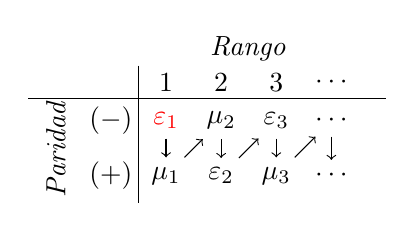
\begin{tikzpicture}[x=0.7cm,y=0.7cm]
    \draw node  at (1,-0.3) {$1$};
    \draw node  at (2,-0.3) {$2$};
    \draw node  at (3,-0.3) {$3$};
    \draw node  at (4,-0.3) {$\cdots$};
    \draw (-1.5,-0.6) -- (5,-0.6);
    \draw node  at (0,-1) {$(-)$};
    \draw node  at (0,-2) {$(+)$};
    \draw (0.5,0) -- (0.5,-2.5);
    \draw node  at (2.5,0.3) {\emph{Rango}};
    \draw node [rotate=90] at (-1,-1.5) {\emph{Paridad}};
    \draw node [red] (node11) at (1,-1) {$\varepsilon_1$};
    \draw node (node12) at (2,-1) {$\mu_2$};
    \draw node (node13) at (3,-1) {$\varepsilon_3$};
    \draw node (node14) at (4,-1) {$\cdots$};
    \draw node (node21) at (1,-2) {$\mu_1$};
    \draw node (node22) at (2,-2) {$\varepsilon_2$};
    \draw node (node23) at (3,-2) {$\mu_3$};
    \draw node (node24) at (4,-2) {$\cdots$};
    %
    \draw[->] (node11) to (node21);
    \draw[->] (node12) to (node22);
    \draw[->] (node13) to (node23);
    \draw[->] (node14) to (node24);
    %
    \draw[->] (node21) to (node12);
    \draw[->] (node22) to (node13);
    \draw[->] (node23) to (node14);
  \end{tikzpicture}
  \caption{Aproximaciones multipolares en orden de importancia. Las
    $\varepsilon_i$ denotan multipolos eléctricos de rango $i$ y las
    $\mu_i$ multipolos magnéticos, donde $i=1$ son dipolos, $i=2$
    cuadrupolos, $i=3$ octupolos, etc.}
  \label{fig:dipolochungo}
\end{marginfigure}










%%% Local Variables:
%%% mode: latex
%%% TeX-master: "../resumen"
%%% End:
